%%%%%%%%%%%%%%%%%%%%%%%%%%%%%%%%%%%%%%%%%
% Large Colored Title Article
% LaTeX Template
% Version 1.1 (25/11/12)
%
% This template has been downloaded from:
% http://www.LaTeXTemplates.com
%
% Original author:
% Frits Wenneker (http://www.howtotex.com)
%
% License:
% CC BY-NC-SA 3.0 (http://creativecommons.org/licenses/by-nc-sa/3.0/)
%
%%%%%%%%%%%%%%%%%%%%%%%%%%%%%%%%%%%%%%%%%

%----------------------------------------------------------------------------------------
%	PACKAGES AND OTHER DOCUMENT CONFIGURATIONS
%----------------------------------------------------------------------------------------

\documentclass[DIV=calc, paper=a4, fontsize=11pt, twocolumn]{scrartcl}	 % A4 paper and 11pt font size

\usepackage{lipsum} % Used for inserting dummy 'Lorem ipsum' text into the template
\usepackage[english]{babel} % English language/hyphenation
\usepackage[protrusion=true,expansion=true]{microtype} % Better typography
\usepackage{amsmath,amsfonts,amsthm} % Math packages
\usepackage[svgnames]{xcolor} % Enabling colors by their 'svgnames'
\usepackage[font=small,labelfont=bf, justification=justified,format=plain]{caption}
\usepackage{booktabs} % Horizontal rules in tables
\usepackage{fix-cm}	 % Custom font sizes - used for the initial letter in the document
\usepackage{soul}
\usepackage{graphicx}
\usepackage{color}
\usepackage[numbers]{natbib}
\usepackage{fancyhdr}
\usepackage[export]{adjustbox}
\usepackage{wrapfig}
\bibliographystyle{abbrv}
%\usepackage{helvet}
%\renewcommand{\familydefault}{\sfdefault}


\usepackage{titlesec}

\usepackage{sectsty} % Enables custom section titles
\allsectionsfont{\color{DarkGoldenrod}\usefont{OT1}{phv}{b}{n}} % Change the font of all section commands

\usepackage{fancyhdr} % Needed to define custom headers/footers
\pagestyle{fancy} % Enables the custom headers/footers
\fancyhf{}

\usepackage{lastpage} % Used to determine the number of pages in the document (for "Page X of Total")

% Headers - all currently empty
\lhead{}
\chead{}
\rhead{}

% Footers
\lfoot{ \includegraphics[scale=0.15,valign=c]{iic.jpg}
               \includegraphics[scale=0.32,valign=c]{harris.png}
              \includegraphics[scale=0.15,valign=c]{ipam.png}
              \includegraphics[scale=0.1,valign=c]{usaid.png}
              \includegraphics[scale=0.23,valign=c]{whrc.png}  
              \includegraphics[scale=0.23,valign=c]{mbl.jpg}           
            }


\renewcommand{\headrulewidth}{0.0pt} % No header rule
\renewcommand{\footrulewidth}{0.4pt} % Thin footer rule

\usepackage{lettrine} % Package to accentuate the first letter of the text
\newcommand{\initial}[1]{ % Defines the command and style for the first letter
\lettrine[lines=3,lhang=0.3,nindent=0em]{
\color{DarkGoldenrod}
{\textsf{#1}}}{}}

%----------------------------------------------------------------------------------------
%	TITLE SECTION
%----------------------------------------------------------------------------------------

\usepackage{titling} % Allows custom title configuration

\newcommand{\HorRule}{\color{DarkGoldenrod} \rule{\linewidth}{1pt} \hrule\vspace{-2em}} % Defines the gold horizontal rule around the title


\pretitle{\vspace{-30pt} \begin{flushleft} \HorRule \fontsize{20}{20} \usefont{OT1}{phv}{b}{n} \color{DarkGreen} \selectfont} % Horizontal rule before the title

\title{{\color{black}IIC Brazil Summer Policy Lab}\\ \vspace{.3cm}Hydropower Construction and Deforestation: Linking Forest Cover to Changes in Water Balance} % Your article title

\posttitle{\par\end{flushleft}\vskip 0.5em} % Whitespace under the title

\preauthor{\begin{flushleft}\large \lineskip 0.5em \usefont{OT1}{phv}{b}{sl} \color{DarkGreen}} % Author font configuration
\author{Soudeep Deb\textsuperscript{1}, Joel Smith\textsuperscript{2}, Ane Alencar\textsuperscript{3}, Isabel Silva\textsuperscript{3} and Michael Coe\textsuperscript{4}\\} % Your name

\postauthor{\footnotesize \usefont{OT1}{phv}{m}{sl} \color{Black} % Configuration for the institution name
\textsuperscript{1}Department of Statistics, University of Chicago, Chicago, IL, USA; sdeb@uchicago.edu\\
\textsuperscript{2}Department of Ecology and Evolution, University of Chicago, Chicago, IL, USA; joelsmith@uchicago.edu\\
\textsuperscript{3}Instituto de Pesquisa Ambiental do Amaz\^ onia, Bras\'{i}lia, Brasil\\
\textsuperscript{4}Woods Hole Research Center, Falmouth, MA, USA
\vspace{-2em}
\par\end{flushleft}\HorRule} % Horizontal rule after the title
\date{} % Add a date here if you would like one to appear underneath the title block

%----------------------------------------------------------------------------------------t

\begin{document}

\maketitle % Print the title
\thispagestyle{fancy} % Enabling the custom headers/footers for the first page 
\initial{H}ydropower construction represents the largest potential driver of deforestation in the Amazon as a result of: (1) Road construction creating access to remote areas; (2) Migrant workers leading to rapid increases in population density; and (3) Infrastructure construction necessary to support this population growth. As of November 2015, 237 dams were planned or under construction in the Brazilian Amazon \cite{castello2015large}. Hydropower construction in the Tapaj\'{o}s River Basin represented one third of this total. The amount of deforested area in the Tapaj\'{o}s River Basin was estimated to be between 42\% and 105\% greater than background rates of deforestation by 2030 (Fig. 1). In early August 2016 the environmental license to build the largest of these dams, the S\~{a}o Luiz do Tapaj\'{o}s, was denied. In addition to future expansion of hydropower throughout the Amazon, 43 dams are still planned for the Tapaj\'{o}s River Basin.

\begin{figure}
  \centering
  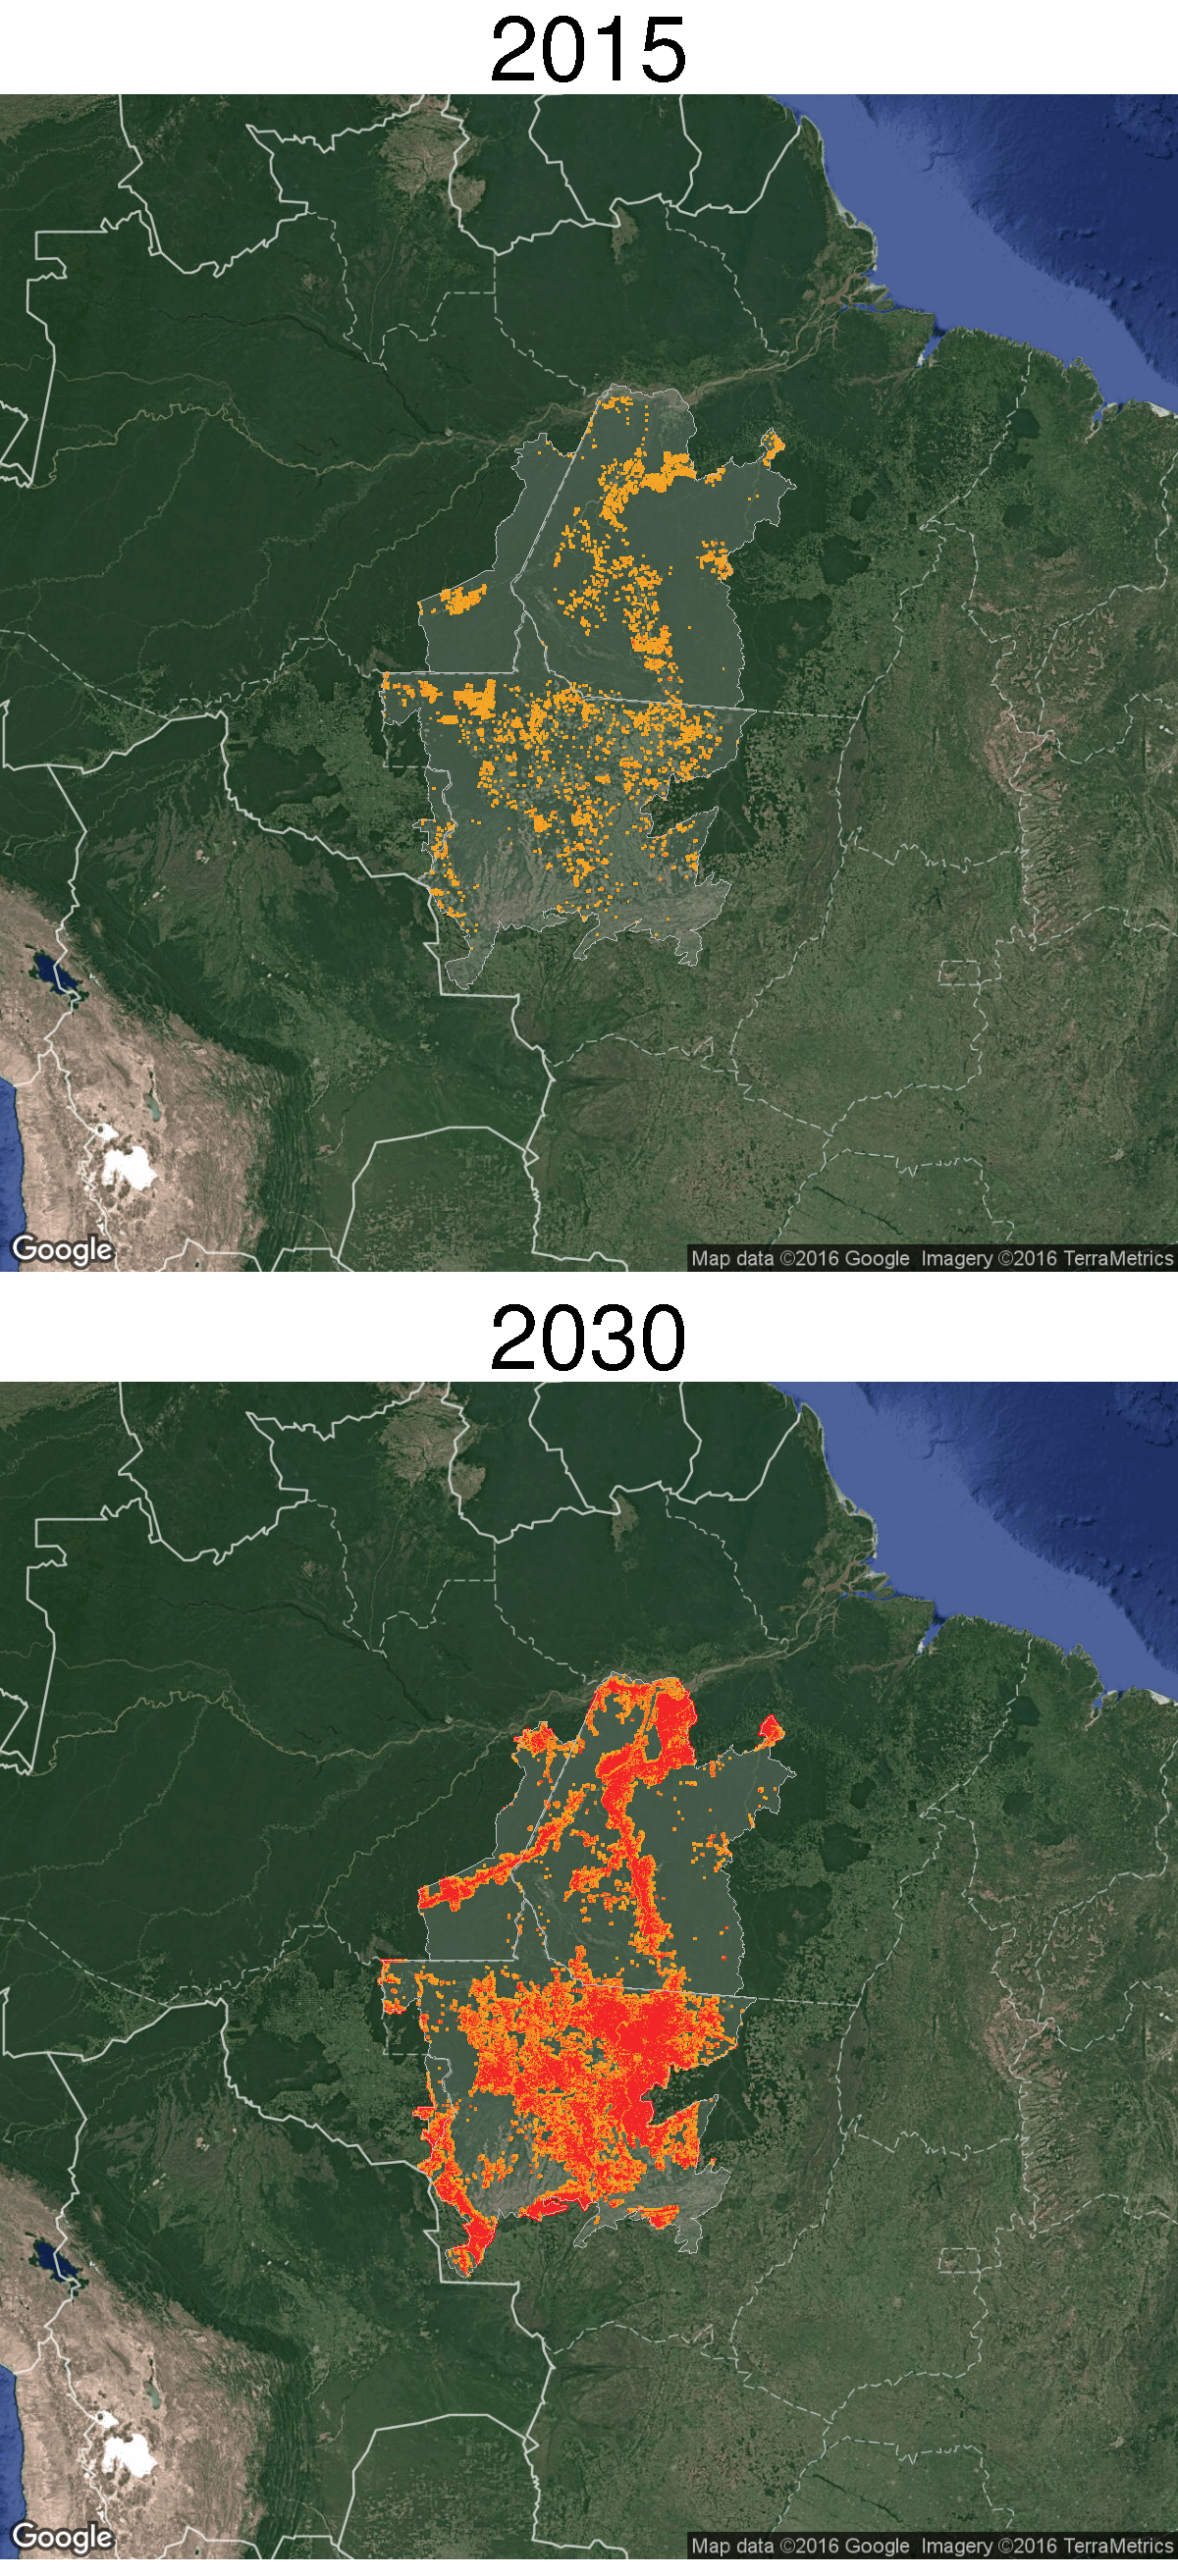
\includegraphics[width=.9\linewidth]{deforest_compare.pdf}
 \caption{Observed deforestation in 2015 and projected deforestation in 2030 among municipalities in the Tapaj\'{o}s river basin.}
  \label{fig:deforest}
\end{figure}

%------------------------------------------------

%\section*{Deforestation Increases Fire Frequency}
%Deforestation leads to increased forest fragmentation and high soil temperatures, both of which contribute to high fire ignition rates \cite{alencar2015landscape, cochrane1999positive}. Current observations suggest a cyclical pattern of continued forest degradation as a result of the following process:
%\begin{itemize}
%\item High temperatures in deforested fields destroys forest edges for hundreds of meters into the forest interior.
%\item As a result of more sunlight in forest edges, grasses invade which leads to higher flammability.
%\item Increased fire frequency on forest edges progressively destroys the forest from the edges to the interior.
%\end{itemize}

%------------------------------------------------

\section*{The Effect of Deforestation on Local and Regional Water Balance}
Rainfall is dependent on both the water vapor being transported from upwind and the local water vapor input via evapo-transpiration (ET). Deforestation is known to have several important negative effects on the cycling of water and the energy in tropical ecosystems. First, pastures and crops absorb less energy from the sun and evaporate less water than forests, dramatically reducing the amount of energy and water returned to the atmosphere. By starving the atmosphere of energy and water local and regional rainfall is decreased \cite{coe2009influence}. As a result of removing water from the atmosphere and changing the energy balance, rainfall is expected to decrease at local and regional scales, with potentially negative consequences for crop production \cite{oliveira2013large}. Next, by changing evaporation and rainfall, river discharge is affected. A forested landscape provides a slow release of water into streams during the dry season. A deforested landscape can result in big changes in the seasonal flow of river water, often with much more in the wet season and much less in the dry season. These types of changes can be especially difficult for consistent hydroelectric power generation and change the ecological function of rivers and streams\cite{coe2011effects}. 

%------------------------------------------------
\section*{Our Question}
How will deforestation in the Tapaj\'{o}s River Basin affect seasonal variability in river discharge, ET and net energy (rainfall potential)? Below we use results from land-surface modeling (IBIS) to quantify the effect of deforestation on the magnitude of change in several water and energy balance characteristics in the Tapaj\'{o}s River Basin \cite{coe2009influence}.
%------------------------------------------------
\section*{Results and Recommendations}
We find that with the current level of deforested area in the Tapaj\'{o}s River Basin (34\%),  the discharge of the Tapaj\'{o}s River is much lower in the dry season, while ET is lower during the rainy season. Similarly, we find that total net energy returned to the atmosphere, which is a driver of rainfall, is strongly decreased by deforestation. We recommend the following policy strategies to avoid or offset these effects:


\renewcommand{\labelitemi}{${\color{DarkGoldenrod}\bullet}$}
\begin{itemize}
\item Hydropower construction undermines its own potential for energy production through the associated deforestation, by creating more seasonally variable source of water. We suggest the use of alternative energy strategies, such as solar and wind energy as much as possible, to maintain the proper functioning of the water cycle.
\item Deforestation in one place can affect rainfall hundreds of miles away potentially affecting crop production and natural ecosystems. Policies to reduce the amount of deforestation that are directly and indirectly associated with dam construction, reduce the costs of forest restoration, and incentivize the maintenance of forested areas should be made a priority. 
\item Some of the costs of enforcement, restoration, and protection should be built into the costs of government funded construction projects.
\end{itemize}


\begin{figure}[h]
\vspace{-3.5em}
  \includegraphics[width=1\linewidth]{SeasonalEffects.pdf}
\vspace{-2em}
 \caption{The effect of deforestation on discharge and ET for each month from year 2000 to 2014. If there were no effect of deforestation we would expect both lines to be flat at a ratio of 1 across all months.}
  \label{fig:deforest}
\vspace{-2em}
\end{figure}

\begin{figure}[h]
\vspace{-1em}
  \includegraphics[width=1\linewidth]{Rnet_rec.pdf}
\vspace{-2em}
 \caption{Difference in net energy (rainfall potential) under the legal limit of deforested area (blue) and observed level of deforestation (red). }
  \label{fig:deforest}

\end{figure}




%----------------------------------------------------------------------------------------


%----------------------------------------------------------------------------------------
%	REFERENCE LIST
%---------------------------------------------------------------------------------------- 
{\scriptsize \bibliography{reference}}

%{\bf \noindent Acknowledgements}\\
%{We thank Isabel Silva from IPAM for access to deforestation data and simulation results.} 
%----------------------------------------------------------------------------------------

\end{document}